\documentclass[class=report, crop=false, 12pt,a4paper]{standalone}
\usepackage{enumitem}
\usepackage{multicol}
\usepackage{graphicx}
\usepackage{float}
\usepackage{amsmath}
\usepackage{amssymb}
\usepackage{mathtools}
\usepackage{siunitx}
\usepackage{commath}
\usepackage{array}
\usepackage{natbib}
\usepackage{booktabs}
\usepackage{multirow}
\usepackage{adjustbox}
\usepackage{mhchem}
\usepackage[a4paper,width=150mm,top=25mm,bottom=25mm]{geometry}
\setlength{\parindent}{0pt}
\begin{document}
\chapter{Materials, Molecules and Chemistry}
\section{Introduction}
\begin{itemize}
	\item Macorscopic response of material depends on their microscopic structure
	\item We need to be able to understand physics from molecular to continuum scales
\end{itemize}
\begin{figure}[H]
	\centering
	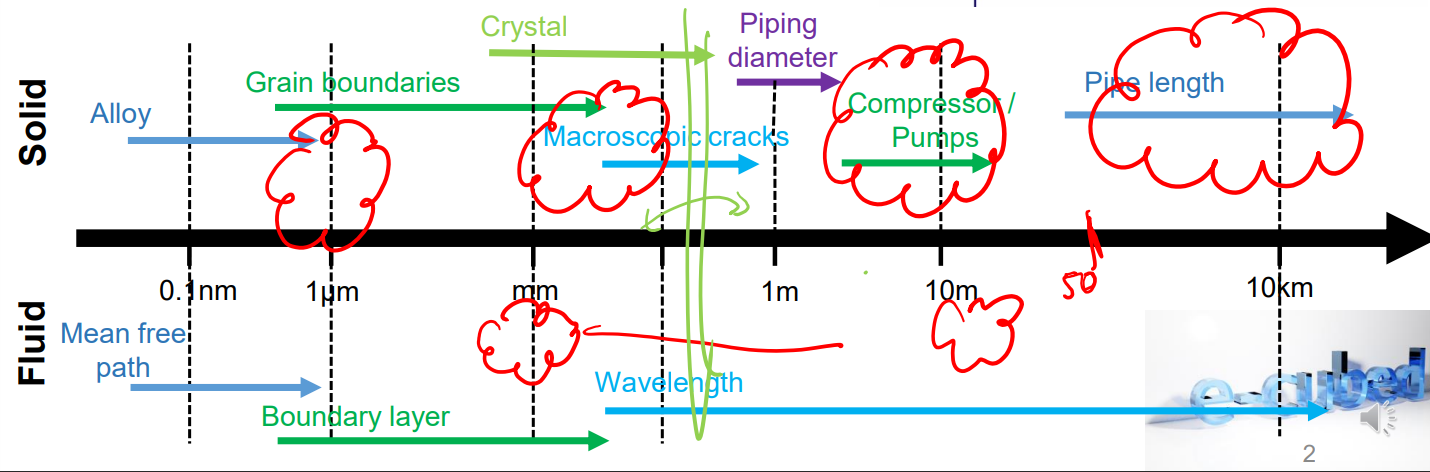
\includegraphics[width = \textwidth]{../img/figure1.png}
	\caption{Pressure pulsation in a piping system}
\end{figure}
\subsubsection{Cascade of length scales}
\begin{table}
\begin{adjustbox}{width=\columnwidth,center}
	\begin{tabular}{@{}lll@{}}
		\toprule
		\textbf{Molecular} & \textbf{Continuum} & \textbf{Structural}\\
		\midrule
		Material is made on this level & Cracks operate on this level & Structures considered at this level\\
		$< \SI{10}{\micro\meter}$ & $\SI{10}{\micro\meter} < x < \SI{10}{\meter}$ & $> \SI{10}{\meter}$\\
		Short range interactions & Long range interactions & Whole scale interactions\\
		Failure / corrosion / chemistry & Tune model - variables change & Long distance interaction \\
		& continuously / smoothly (can account & - vibration (waves transporting energy)\\
		& for discontinuous behaviour, e.g. crack) & \\
		\bottomrule
	\end{tabular}
\end{adjustbox}
\caption{Cascade of length scales}
\end{table}
\subsection{Compelxity of the problem at different length scales}
Complexity of representation changes with the scale.
\begin{figure}[H]
	\centering
	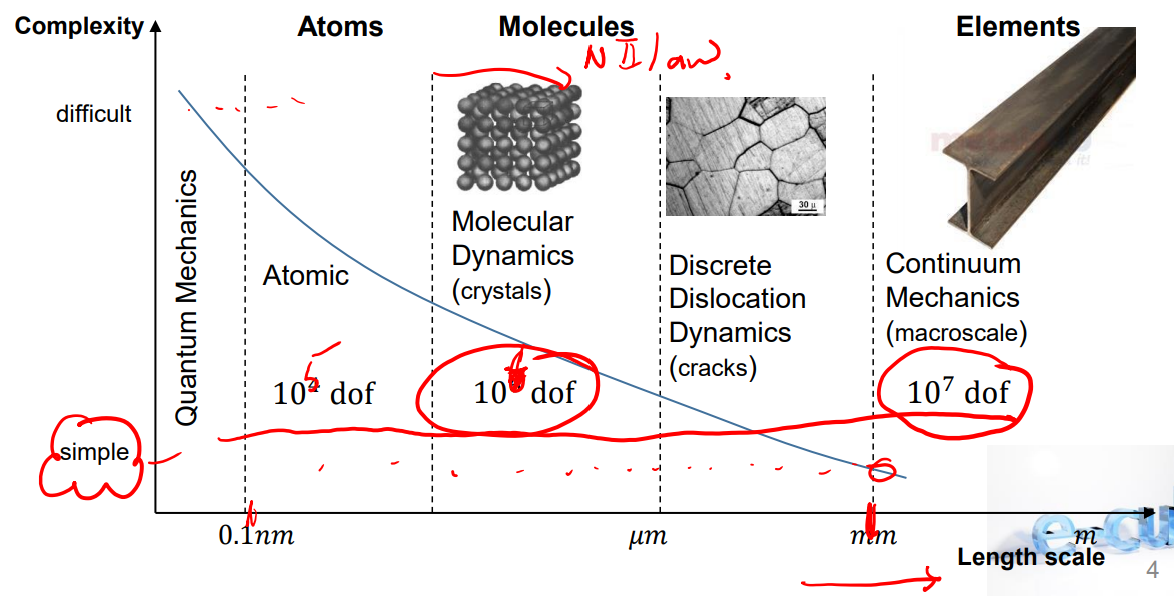
\includegraphics[width = \textwidth]{../img/figure2.png}
	\caption{Graph to show complexity against scale.}
\end{figure}
\subsection{Why focus on small scales?}
\begin{itemize}
	\item Small scale defects lead to crack initiation and propagation under external loading
	\item Failure can be corrected by changing material properties, for example, toughness
	\item Source of defects: complex chemical process (chemistry / corrosion) leads to corrosion at the surface
	\item Macroscale process is linked to microscale action
	\item Hypersonic flow - ionisation is non-continuum effect
	\item Analogy between defective liquids / solids
\end{itemize}
Note: turbulence is controllbed by small vortices.
\subsubsection{Micrograph}
\begin{table}
	\centering
	\begin{tabular}{@{}ll@{}}
		\toprule
		\textbf{Domain} & \textbf{Process}\\
		\midrule
		Bulk & Plasticity\\
		Internal boundary & Hydrogen embrittlement - \\
		& plastic deformation / slip\\
		External boundary & Corrosion - chemistry\\
		\bottomrule
	\end{tabular}
	\caption{Micrograph}
\end{table}
\begin{figure}[H]
	\centering
	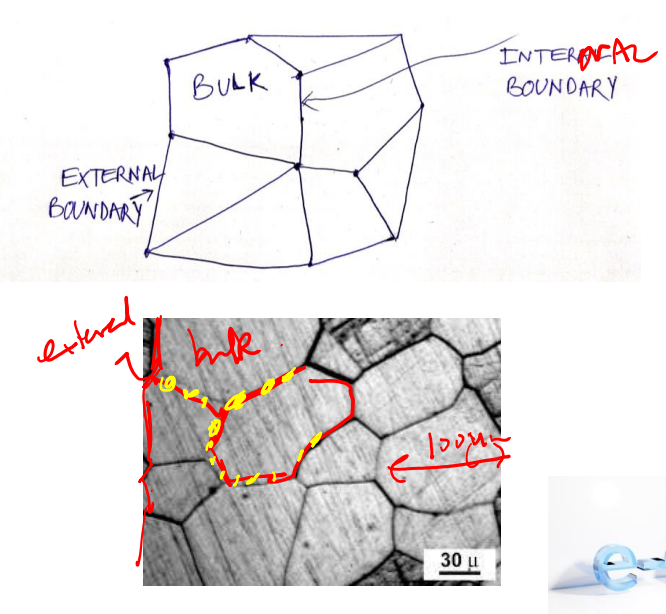
\includegraphics[width = 0.5\textwidth]{../img/figure3.png}
	\caption{Graph to show complexity against scale.}
\end{figure}
\subsubsection{Internal grain processes}
\begin{figure}[H]
	\centering
	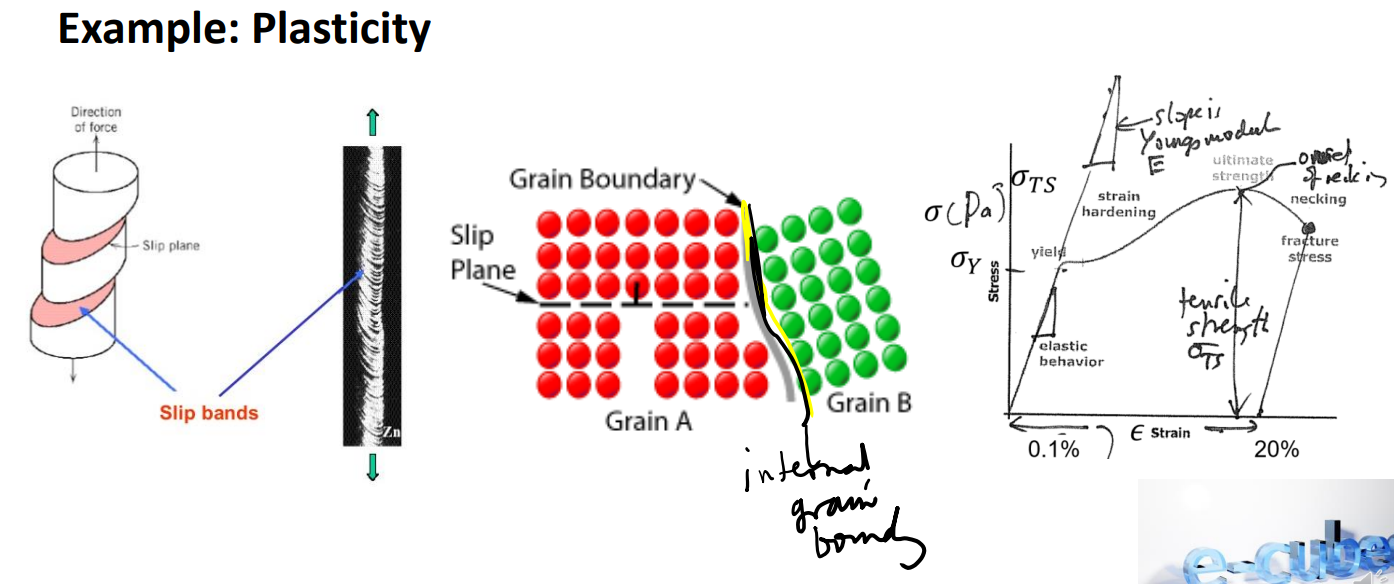
\includegraphics[width = 0.5\textwidth]{../img/figure4.png}
	\caption{Example of plasticity from internal grain process level.}
\end{figure}
\subsubsection{Internal boundary (hydrogen embrittlement - plastic deformation / slip)}
\begin{figure}[H]
	\centering
	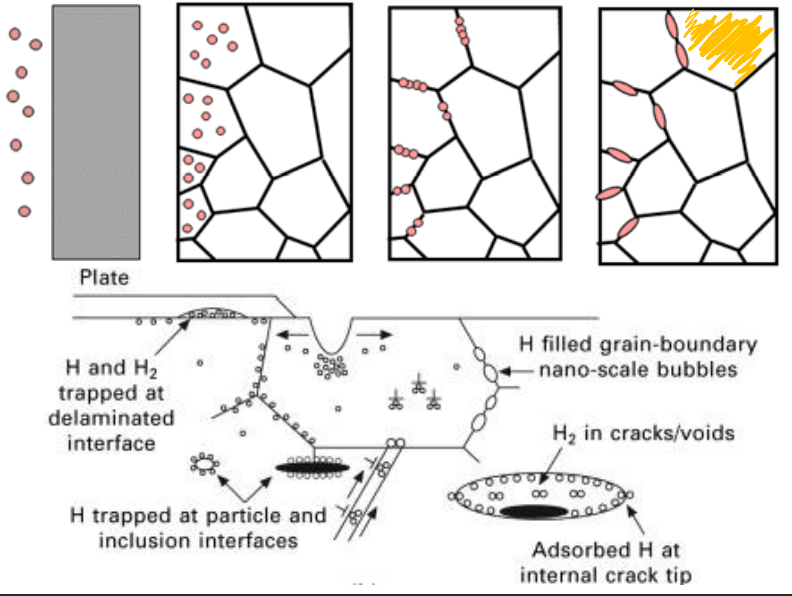
\includegraphics[width = 0.5\textwidth]{../img/figure5.png}
	\caption{Hydrogen embrittlement - plastic deformation / slip}
\end{figure}
\subsubsection{External boundary (corrosion)}
Corrosion happens over a long time and a range of scales. We need to understand how ions move around and interact with materials.
\begin{gather}
	\ce{Fe2 + (ag) + 2OH(ag) -> Fe(OH)_{2(s)}}\\
	\ce{4Fe(OH)_{2(s)} + O_{2(g)} + 2H2O_{(l)} -> Fe(OH)_{3(s)}}
\end{gather}
\begin{figure}[H]
	\centering
	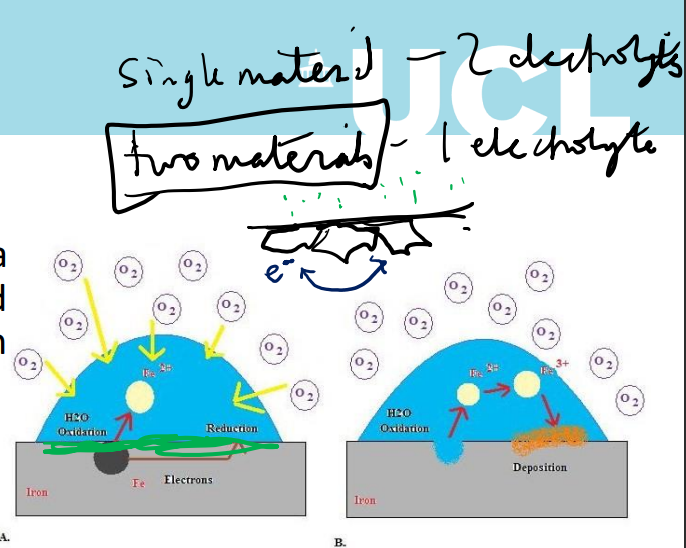
\includegraphics[width = 0.5\textwidth]{../img/figure6.png}
	\caption{Rust corrosion from grain boundary level.}
\end{figure}
\section{Categorisation of matter}
\begin{table}
	\centering
	\begin{tabular}{@{}lll@{}}
		\toprule
		\textbf{Matter} & \textbf{Modelling approach} & \\
		\midrule
		Solid & Atomistic & Continuum\\
		Gas & Kinetic theory & Continuum\\
		Liquid & Molecular & Continuum\\
		\bottomrule
	\end{tabular}
	\caption{Categorisation of matter}
\end{table}
Switch between states are due to $p$, $V$ and $T$ and is represented by phase diagram. States of matter have been part of most religious and scientific texts for the last two thousand years, with water (aqua), fire (ignis), air (aer) and earth (terra) with the fifth being the void.
\section{Atomistic view of matter}
Typical length scale:
\begin{itemize}
	\item Diameter of atom is \SI{0.1}{\nano\meter} = \SI{1e-10}{\meter} = \SI{1}{angstrom}
	\item Nucleus diameter is \SI{1e-15}{\meter} (hydrogen) to \SI{15e-15}{\meter} (uranium-238)
\end{itemize}
\subsection{Bulk characteristic of materials}
The aim is to understand the relationship between the macrostructure and the microstructure. Key measures are:
\begin{itemize}
	\item Young's modulus $E = \left. \frac{\dif \sigma}{\dif \varepsilon} \right|_{\varepsilon \rightarrow 0}$
	\item Tensile stress: $\sigma_{TS}$
	\item Yields stress: $\sigma_{Y}$
	\item Ductility: $\epsilon_{T}$
\end{itemize}
It is important to understand the following:
\begin{table}
	\centering
	\begin{tabular}{@{}lll@{}}
		\toprule
		\textbf{Properties} & &\textbf{Definition}\\
		\midrule
		Elastic modulus & $E$ (\si{\pascal}) & Measure of material resistance to deformation.\\
		Yield stress & $\sigma_Y$ (\si{\pascal}) & Measure of stress at which the elastic behaviour\\
		& & disappears and plastic behaviour initiates.\\
		Hardness & HBW & Measure of material resistance to indentation\\
		Creep & & Time-dependant deformation at high temperature\\
		& & and constant stress.\\
		Toughness & $K$ (\si{\joule\per\meter\cubed}) & Resistance to crack propagation.\\
		Ductility & $\epsilon_T$ & Material's ability to undergo plastic deformation.\\
		\bottomrule
	\end{tabular}
	\caption{Key points on material properties}
\end{table}
How are they related to the microstrucure? 
\subsection{Newtonian model of matter}
Useful for biological, physical problems, solids, liquids and gases. This is based on a description of matter as a collection of point particles, an approach that is useful for gases, liquid and solids. The dynamics of the i-th molecule is:
\begin{gather}
	\underline{F}_i = \sum_{j,j} \neq \nabla U\left(x_i,x_j\right)
\end{gather}
Located at point $\underline{x}_i$ whose dynamics are:
\begin{gather}
	m_i \dfrac{\dif \underline{v}_i}{\dif t} = \underline{F}_i\\
	\underline{v}_i = \frac{\dif \underline{x}_i}{\dif t}
\end{gather}
The formulation requires the form of the interaction stated using the Lennard-Jones 6-12 potential:
\begin{gather}
	U = 4 \epsilon \left(\left(\frac{\sigma}{r}\right)^{12} - \left(\frac{\sigma}{r}\right)^6\right) + \dots
\end{gather}
The difficultuy is that neighbourhood lists are kept and only sum over local interaction of molecules.
\begin{itemize}
	\item Not hard collision
	\item Time stepping fixed
	\item Potentials can be empirical or chosen to now slow down calculations
\end{itemize}
\begin{gather}
	U = U_{stretch} + U_{bend} + U_{torsion} + U_{vanderWaal} + U_{electro} + U_{cross}
\end{gather}
Research gaps:
\begin{itemize}
	\item Link between continuum and molecular
	\item Quantim - mechanical models
\end{itemize}
\subsection{Vibrational modes and energy}
Mechanical representation of matter. Molecules interact with their neighbours and fields. Interaction may be quite far, particularly when charges are important. We are familiar with how degrees of freedom influence properties of a gas, especially through the isentropic index. Energy is stored in various modes of vibration e.g. gas. This is called classical molecular dynamics.
\subsection{Molecular description of material properties}
\subsubsection{Primary bonds}
Ionic and covalent bonds are exteremes with most (electron distribution) bonds lying between (polar covalent)
\begin{figure}[H]
	\centering
	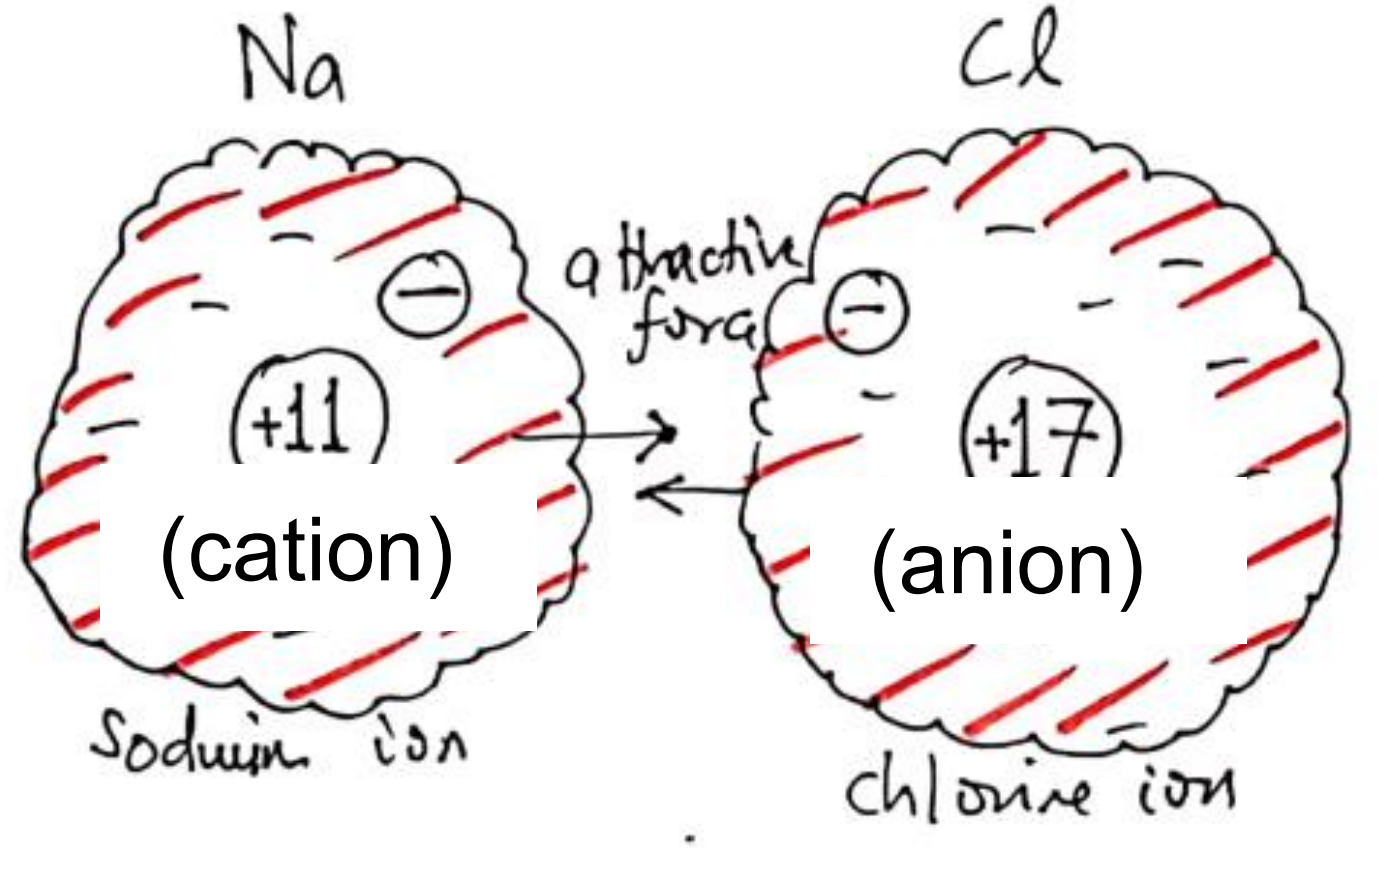
\includegraphics[width = 0.5\textwidth]{../img/figure7.png}
	\caption{Ionic bond (electrovalence)}
\end{figure}
\begin{gather}
	F = \frac{q_1 q_2}{4\pi \epsilon_0 r^2}\\
	U = U_i - \frac{q^2}{4\pi\epsilon_0 r} + \frac{B}{r^n}
\end{gather}
\begin{figure}[H]
	\centering
	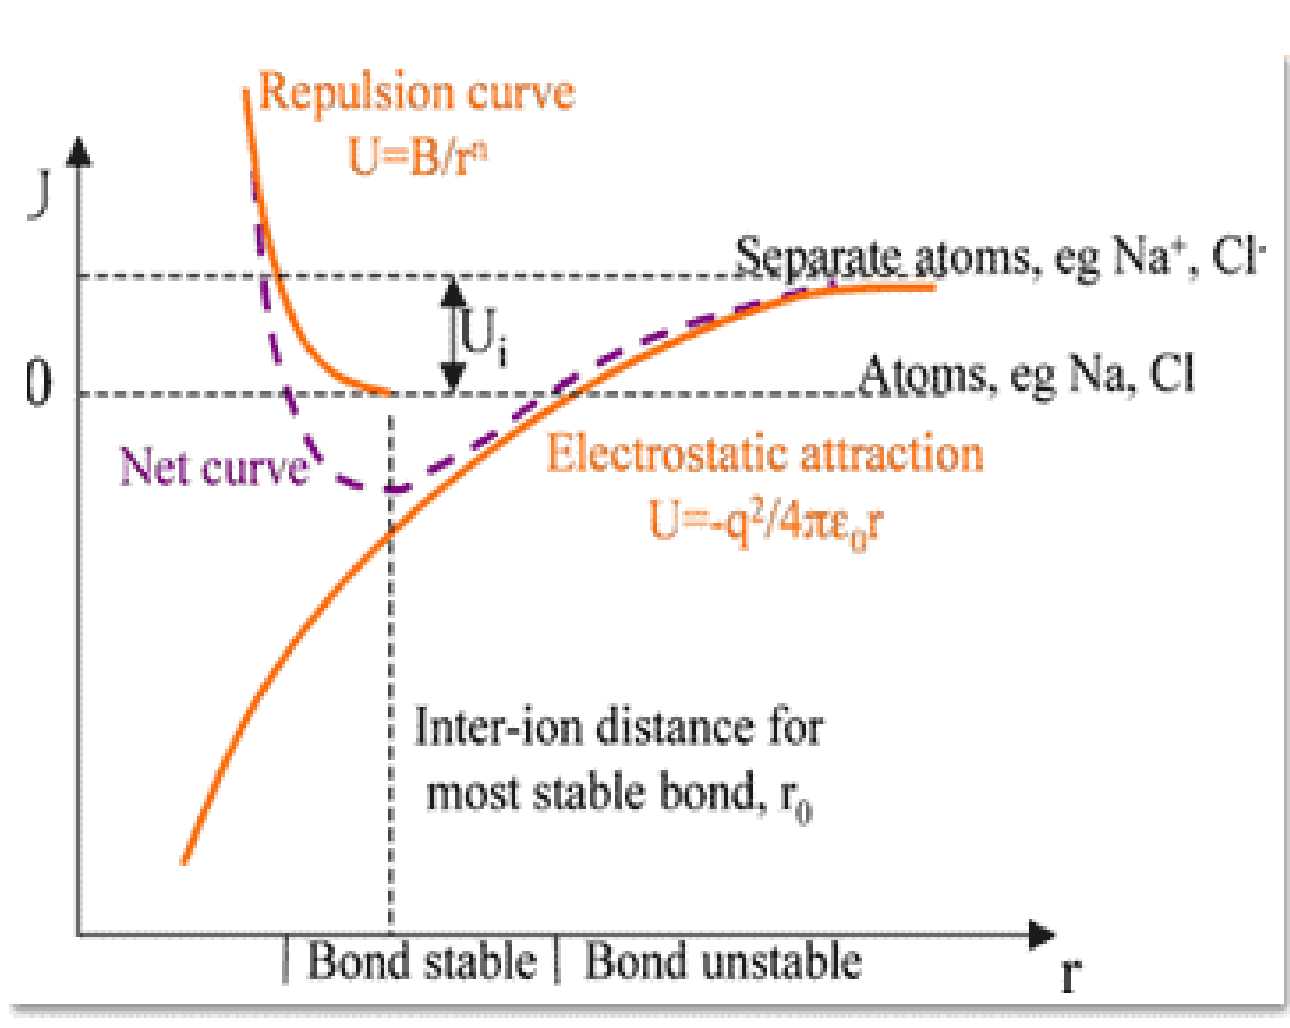
\includegraphics[width = 0.5\textwidth]{../img/figure8.png}
	\caption{Bond stability.}
\end{figure}
\begin{figure}[H]
	\centering
	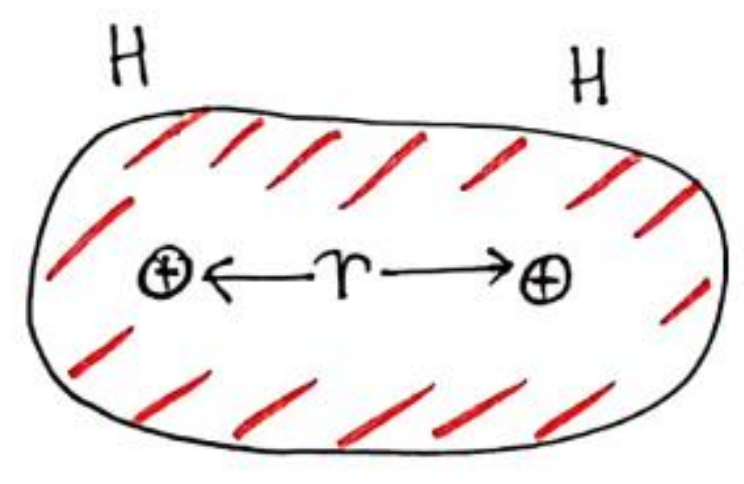
\includegraphics[width = 0.5\textwidth]{../img/figure9.png}
	\caption{Covalent bond (covalence). Note the overlap of electron orbit.}
\end{figure}
\begin{gather}
	U = -\frac{A}{r^m} + \frac{B}{r^n}, \, m<n
\end{gather}
\begin{figure}[H]
	\centering
	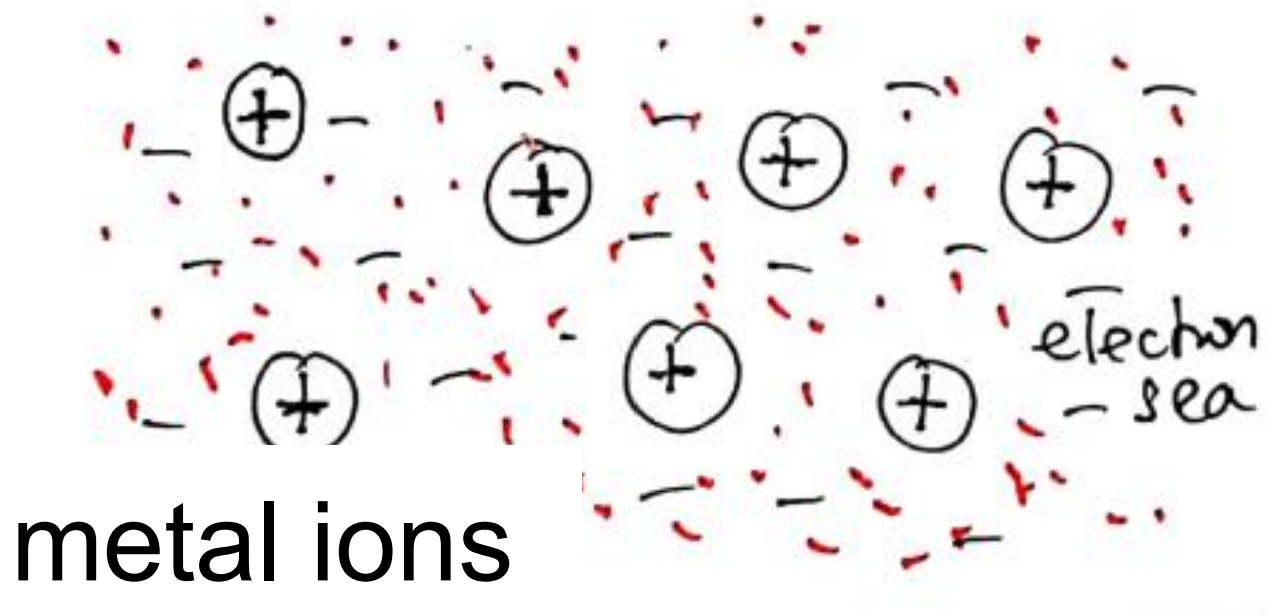
\includegraphics[width = 0.5\textwidth]{../img/figure10.png}
	\caption{Metallic bond (electron cloud).}
\end{figure}
\begin{gather}
	e = \SI{1.6e-19}{C}\\
	\epsilon_0 = \SI{8.8e-12}{Nm^2C^{-2}}\\
	\SI{1}{eV} = \SI{1.6e-19}{J}
\end{gather}
\end{document}